\section{Results and Analysis}
\label{sec:results}
% In this section, we present the experimental results of our proposed QAMA (Quantization Aware Matryoshka Adaptation) approach using two different models: Modern BERT (MB) \cite{modernbert, nussbaum2024nomic} and MiniLM \cite{minilm, reimers-2019-sentence-bert}. 
We evaluate the performance across various embedding dimensions and quantization levels to demonstrate the effectiveness of our methods in reducing storage requirements and improving retrieval speed while maintaining high accuracy.


Tables~\ref{tab:mb_main_results} and~\ref{tab:minilm_main_results} compare the performance of Modern BERT (MB) and MiniLM at various quantization levels and dimensions, using nDCG@10 average across multiple datasets as the primary metric. 
\paragraph{Key Insights:}
\begin{itemize}
    \item \textbf{2-bit Quantization Nears FP32 Performance:} As shown in the ablation studies, 2-bit quantization retains around 95--98\% of FP32 performance, demonstrating its effectiveness in preserving semantic information.
    \item \textbf{Hybrid Quantization Efficiency:} The Hybrid approach offers additional storage savings while maintaining performance close to 2-bit, as evidenced by the ablation results.
    \item \textbf{Role of Matryoshka Loss:} The introduction of Matryoshka Loss significantly enhances performance, particularly at lower dimensions, by concentrating essential information in early dimensions.
\end{itemize}

\begin{table}[ht]
\caption{Performance of Modern BERT (MB) with different quantization levels and embedding dimensions.}
\label{tab:mb_main_results}
\centering
\begin{tabular}{lccccc}
\toprule
\textbf{Dimension} & \textbf{1-bit} & \textbf{1.5-bit} & \textbf{Hybrid Quant} & \textbf{2-bit} & \textbf{FP32} \\
\midrule
768 & 0.4381 & 0.4536 & 0.4680 & 0.4687 & 0.4720 \\
384 & 0.4167 & 0.4429 & 0.4509 & 0.4593 & 0.4695 \\
256 & 0.3691 & 0.4228 & 0.4465 & 0.4513 & 0.4680 \\
192 & 0.3285 & 0.3901 & 0.4245 & 0.4327 & 0.4512 \\
96 & 0.2908 & 0.3455 & 0.3850 & 0.3919 & 0.4247 \\
\bottomrule
\end{tabular}
\end{table}

\begin{table}[ht]
\caption{Performance of MiniLM with different quantization levels and embedding dimensions.}
\label{tab:minilm_main_results}
\centering
\begin{tabular}{lccccc}
\toprule
\textbf{Dimension} & \textbf{1-bit} & \textbf{1.5-bit} & \textbf{Hybrid Quant} & \textbf{2-bit} & \textbf{FP32} \\
\midrule
384 & 0.3839 & 0.4101 & 0.4160 & 0.4185 & 0.4286 \\
192 & 0.3724 & 0.3923 & 0.4017 & 0.4109 & 0.4219 \\
128 & 0.3571 & 0.3814 & 0.3865 & 0.3917 & 0.3963 \\
96 & 0.3417 & 0.3649 & 0.3695 & 0.3712 & 0.3792 \\
48 & 0.2687 & 0.2871 & 0.2919 & 0.2897 & 0.3014 \\
\bottomrule
\end{tabular}
\end{table}

Note that for Modern BERT, with dimension FP32, and dimension as 768 (original dimension), the NDCG@10 is 0.4720 and this was using the original model with no changes. 
For MiniLM, with dimension FP32, and dimension as 384 (original dimension), the NDCG@10 is 0.4286 and this was using the original model with no changes.
From the results, we observe that our proposed QAMA framework achieves competitive performance compared to the full-precision (FP32) embeddings, even at significantly reduced storage sizes. 
For instance, the 2-bit quantized embeddings at 384 dimensions achieve an nDCG@10 of 0.4593 with Modern Bert and 0.4185 with MiniLM, which is close to the FP32 performance while reducing the storage requirements substantially.
Although slightly behind pure 2-bit in accuracy, Hybrid Quant offers additional storage savings (\(\approx 1{-}4\%\) more than 2-bit) while keeping performance within 1--2\% of the best quantized results. 


% \subsection{Impact of Quantization Levels}
% \label{sec:quantization_levels}

% We further analyze the impact of different quantization levels on the performance. 
% Figure~\ref{fig:quantization_impact_mb} illustrate the performance across different quantization levels for MB and MiniLM models, respectively.

% \begin{figure}[ht]
%     \centering
%     % \includegraphics[width=0.8\linewidth]{figures/quantization_impact.pdf}
%     \caption{Impact of quantization levels on performance for Modern BERT (MB) and MiniLM across different dimensions.}
%     \label{fig:quantization_impact_mb}
% \end{figure}


Our results show that increasing the quantization level (from 1-bit to 2-bit) consistently improve performance, highlighting the trade-off between storage efficiency and model accuracy. 
The Hybrid Quantization approach, which uses different quantization levels for different embedding dimensions, achieves performance close to 2-bit quantization while offering better storage efficiency  (typically within about 1--2\% of the 2-bit nDCG@10). 
For example, at 384 dimensions in Modern BERT, Hybrid Quant yields 0.4509 nDCG@10 compared to 0.4593 for 2-bit, recovering about 98.2\% of the latter's performance, while saving approximately 2\% additional storage. 
% More generally across our ablations, we observe extra storage savings of roughly 1--4\% compared to pure 2-bit quantization.

\subsection{Effect of Embedding Dimensions}
\label{sec:dimension_effect}

Figure~\ref{fig:dimension_impact_mb} show that higher dimensions generally yield stronger performance due to increased representational capacity. However, our methods maintain competitive accuracy at lower dimensions.
% ------------------------------------------------------------------------
% (4) Turn generic statements into strong statements referencing thresholds from the insights
% ------------------------------------------------------------------------
In particular, the ablation results highlight that, at around 192 dims for MB or 96 dims for MiniLM, the Matryoshka Loss and Orthogonality Regularization become increasingly critical (see Table~\ref{tab:mb_ablation_192} and Table~\ref{tab:minilm_ablation_96}). 
For example, MB at 192 dims with 2-bit quantization retains 0.4327 nDCG@10, compared to 0.4512 for FP32 (i.e., around 96\% of the full-precision performance). 
At lower dimensions, Matryoshka Loss becomes critical in preserving performance by ensuring hierarchical information encoding.
% This capability—preserving semantic effectiveness even in a lower-dimensional space—emerges from the synergy of hierarchical representation learning plus the advanced regularizations.
\begin{figure}[ht]
    \centering
    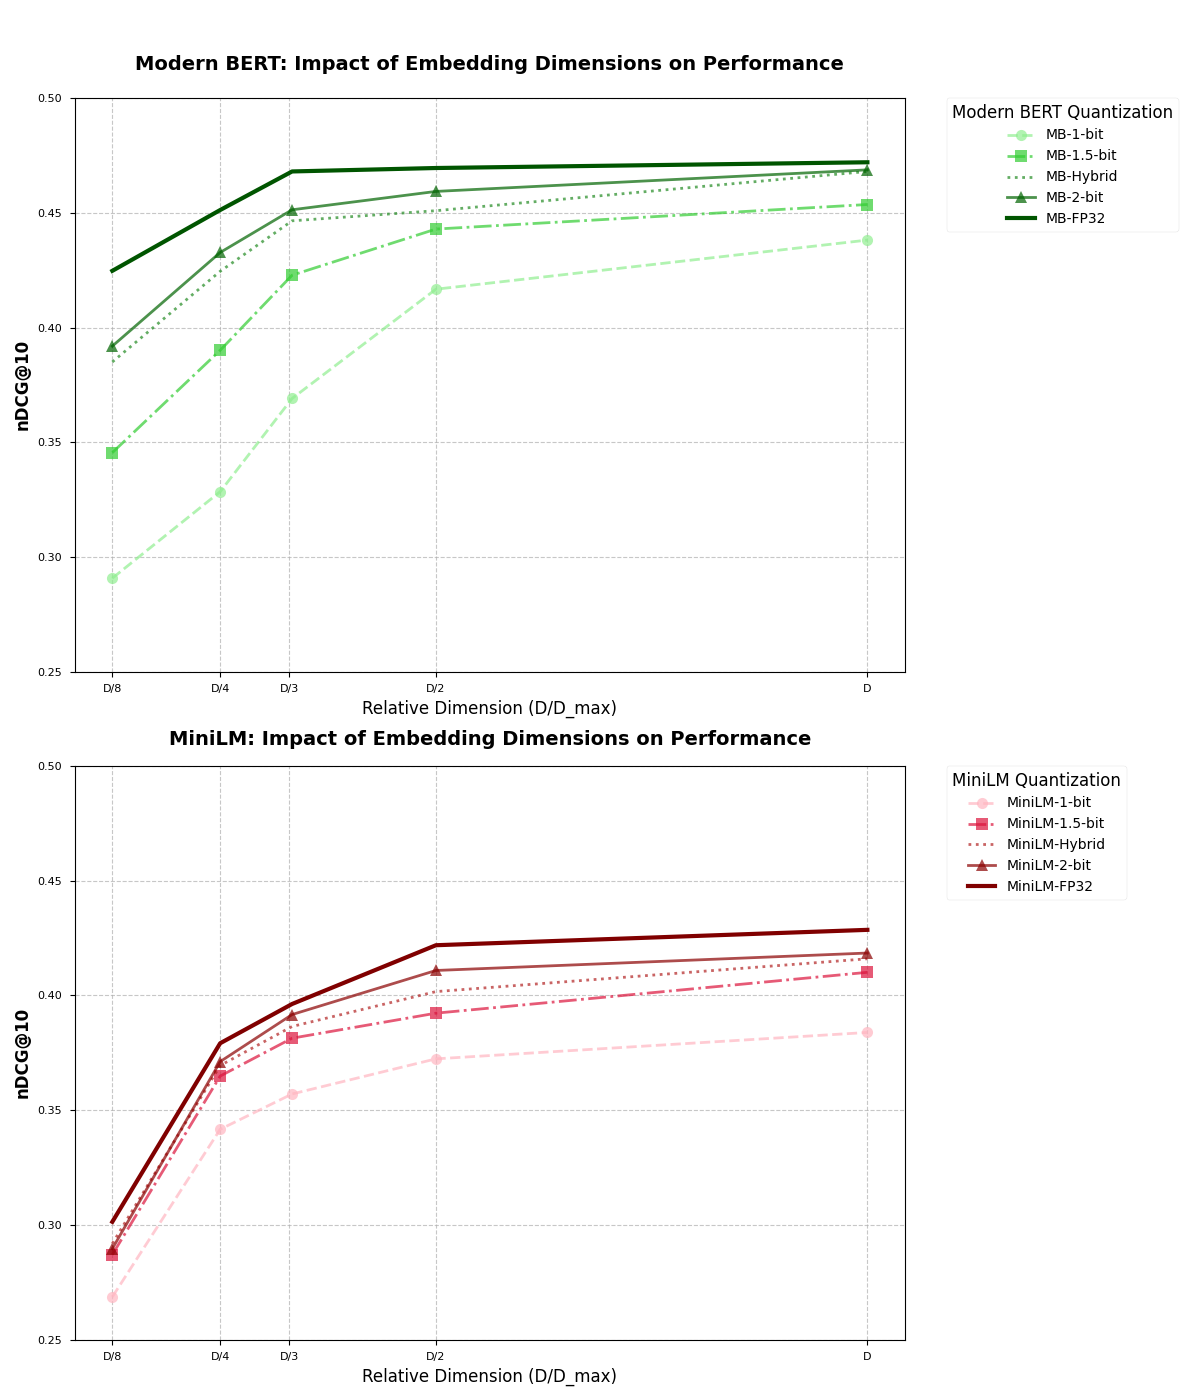
\includegraphics[width=0.8\linewidth]{result_fig_1.png}
    \caption{Impact of embedding dimensions on performance for Modern BERT (MB) and MiniLM model across different quantization levels.}
    \label{fig:dimension_impact_mb}
\end{figure}
These results illustrate that while higher dimensions generally improve performance, our proposed methods enable lower-dimensional embeddings to achieve competitive results, which is beneficial for resource-constrained environments.

\subsection{Ablation Studies}
\label{sec:ablation_summaries}

To evaluate the contribution of each component in our proposed methodology, we perform ablation studies on the MB and MiniLM models at two embedding dimensions each. 
Specifically, we consider dimensions 384 and 192 for the MB model, and dimensions 192 and 96 for the MiniLM model. 
Tables~\ref{tab:mb_ablation_384} and~\ref{tab:mb_ablation_192} present the ablation results for the MB model, while Tables~\ref{tab:minilm_ablation_192} and~\ref{tab:minilm_ablation_96} show the results for the MiniLM model.
We highlight a few \emph{important} observations here:
\begin{itemize}
    \item \textbf{Matryoshka Loss Yields Large Jumps in Lower Dimensions:} E.g., for MiniLM at 96 dims, final performance doubles from \textit{Thresholds Only} to \textit{+ MVC + Orthogonality + IB} (Table~\ref{tab:minilm_ablation_96}). This underscores that hierarchical training is essential when dimension is aggressively reduced.
    \item \textbf{Adaptive Variance Control as a Final “Booster” Step:} In each table, AVC tends to add a 2--4\% relative improvement. This mechanism is vital for preventing degenerate embeddings in scenarios with both low bits and low dimensions.
    % \item \textbf{Orthogonality and Bottleneck Synergy:} These regularizations spread out distinct features among the newly added dimensions (Orthogonality) while forcing early dimensions to capture the most crucial semantic content (Info Bottleneck).
% \end{itemize}

% \paragraph{Model-Specific Observations:}
% \begin{itemize}
    \item \textbf{MB vs. MiniLM:} MB generally retains better performance at higher dimensions, while MiniLM benefits significantly from the matryoshka methods, indicating the approach's adaptability across different architectures.
    \item \textbf{Sensitivity to Compression:} MB shows resilience to dimensional downscaling, whereas MiniLM exhibits faster trade-off declines, reflecting differences in model architecture.
\end{itemize}

\begin{table}[ht]
\caption{Ablation study for MB model at 384 dimensions.}
\label{tab:mb_ablation_384}
\centering
\resizebox{0.98\columnwidth}{!}{
\begin{tabular}{lccccc}
\toprule
\textbf{Training Components} & \textbf{1-bit} & \textbf{1.5-bit} & \textbf{Hybrid Quant} & \textbf{2-bit} & \textbf{FP32} \\
\midrule
Thresholds Only                          & 0.3900  & 0.4250  & 0.4358  & 0.4370  & - \\
+ Trainable FFN Transform               & 0.3922  & 0.4275  & 0.4380  & 0.4390  & 0.4410 \\
+ Quantization Loss                      & 0.3945  & 0.4298  & 0.4402  & 0.4415  & - \\
+ Matryoshka Loss                        & 0.3998  & 0.4318  & 0.4410  & 0.4425  & 0.4632 \\
+ Orthogonality Regularization           & 0.4012  & 0.4329  & 0.4430  & 0.4440  & 0.4645 \\
+ Information Bottleneck Regularization  & 0.4025  & 0.4340  & 0.4442  & 0.4455  & 0.4658 \\
+ Adaptive Variance Control              & \textbf{0.4167}  & \textbf{0.4429}  & \textbf{0.4509}  & \textbf{0.4593}  & \textbf{0.4695} \\
\bottomrule
\end{tabular}
}
\end{table}

\begin{table}[ht]
\caption{Ablation study for MB model at 192 dimensions.}
\label{tab:mb_ablation_192}
\centering
\resizebox{0.98\columnwidth}{!}{
\begin{tabular}{lccccc}
\toprule
\textbf{Training Components} & \textbf{1-bit} & \textbf{1.5-bit} & \textbf{Hybrid Quant} & \textbf{2-bit} & \textbf{FP32} \\
\midrule
Thresholds Only                          & 0.2900  & 0.3550  & 0.3755  & 0.3850  & - \\
+ Trainable FFN Transform               & 0.2922  & 0.3575  & 0.3778  & 0.3872  & 0.3900 \\
+ Quantization Loss                      & 0.2943  & 0.3597  & 0.3801  & 0.3893  & - \\
+ Matryoshka Loss                        & 0.3107  & 0.3732  & 0.3945  & 0.4050  & 0.4405 \\
+ Orthogonality Regularization           & 0.3125  & 0.3752  & 0.3964  & 0.4068  & 0.4422 \\
+ Information Bottleneck Regularization  & 0.3142  & 0.3770  & 0.3983  & 0.4087  & 0.4440 \\
+ Adaptive Variance Control              & \textbf{0.3285}  & \textbf{0.3901}  & \textbf{0.4245}  & \textbf{0.4327}  & \textbf{0.4512} \\
\bottomrule
\end{tabular}
}
\end{table}


\begin{table}[ht]
\caption{Ablation study for MiniLM model at 192 dimensions.}
\label{tab:minilm_ablation_192}
\centering
\resizebox{0.98\columnwidth}{!}{
\begin{tabular}{lccccc}
\toprule
\textbf{Training Components} & \textbf{1-bit} & \textbf{1.5-bit} & \textbf{Hybrid Quant} & \textbf{2-bit} & \textbf{FP32} \\
\midrule
Thresholds Only                         & 0.2947 & 0.3205 & 0.3260 & 0.3324 & - \\
+ Trainable FFN Transform              & 0.3112 & 0.3538 & 0.3645 & 0.3753 & 0.3841 \\
+ Quantization Loss                     & 0.3267 & 0.3661 & 0.3773 & 0.3883 & - \\
+ Matryoshka Loss                       & 0.3318 & 0.3709 & 0.3821 & 0.3922 & 0.3996 \\
+ Orthogonality Regularization          & 0.3354 & 0.3741 & 0.3850 & 0.3940 & 0.4019 \\
+ Information Bottleneck Regularization & 0.3389 & 0.3768 & 0.3876 & 0.3961 & 0.4035 \\
+ Adaptive Variance Control             & \textbf{0.3724} & \textbf{0.3923} & \textbf{0.4017} & \textbf{0.4109} & \textbf{0.4219} \\
\bottomrule
\end{tabular}
}
\end{table}

\begin{table}[ht]
\caption{Ablation study for MiniLM model at 96 dimensions.}
\label{tab:minilm_ablation_96}
\centering
\resizebox{0.98\columnwidth}{!}{
\begin{tabular}{lccccc}
\toprule
\textbf{Training Components} & \textbf{1-bit} & \textbf{1.5-bit} & \textbf{Hybrid Quant} & \textbf{2-bit} & \textbf{FP32} \\
\midrule
Thresholds Only                          & 0.2050 & 0.2330 & 0.2375 & 0.2428 & - \\
+ Trainable FFN Transform               & 0.2250 & 0.2570 & 0.2715 & 0.2860 & 0.3340 \\
+ Quantization Loss                      & 0.2640 & 0.3017 & 0.3161 & 0.3304 & - \\
+ Matryoshka Loss                        & 0.3100 & 0.3350 & 0.3450 & 0.3550 & 0.3600 \\
+ Orthogonality Regularization           & 0.3150 & 0.3380 & 0.3480 & 0.3575 & 0.3625 \\
+ Information Bottleneck Regularization  & 0.3175 & 0.3400 & 0.3500 & 0.3590 & 0.3640 \\
+ Adaptive Variance Control              & \textbf{0.3417} & \textbf{0.3649} & \textbf{0.3695} & \textbf{0.3712} & \textbf{0.3792} \\
\bottomrule
\end{tabular}
}
\end{table}

\textbf{Performance Across Dimensions and Impact of Dimensional Reduction:}
Our methods demonstrate remarkable resilience to dimensional reduction while maintaining competitive performance across different scales. 
At higher dimensions, the MB model with 2-bit quantization achieves an nDCG@10 of 0.4687 at 768 dimensions, close to the FP32 performance of 0.4720 (99.3\% retained). 
When reducing to 384 dimensions, it maintains 0.4593 (97.3\% of FP32), and even at 192 dimensions still achieves 0.4327 (96\% of its corresponding FP32 score of 0.4512).

The effectiveness of our dimensional reduction approach is particularly evident in the step-wise degradation patterns. 
For MB at 2-bit quantization, halving dimensions from 384 to 192 results in only a 6\% relative drop (0.4593 to 0.4327), while the corresponding FP32 models show a similar 3.9\% decrease (0.4695 to 0.4512). 
This near-parallel degradation suggests our quantization effectively preserves the inherent information hierarchy across dimensions.

MiniLM exhibits similar robustness: at 2-bit quantization, performance decreases from 0.4185 at 384 dimensions to 0.4109 at 192 dimensions (just 1.8\% drop), and to 0.3712 at 96 dimensions (about 10\% reduction from 192 dimensions). 
Notably, when compared to their respective FP32 baselines, the 2-bit models consistently retain 95-97\% of full-precision performance across all dimension levels (e.g., 0.3712 vs 0.3792 at 96 dimensions, 97.9\% retained).
% The ablation studies further validate this dimensional robustness. For instance, 
In Table~\ref{tab:minilm_ablation_96}, even at aggressive 96-dimension compression, the full pipeline (including Matryoshka Loss, Orthogonality, Information Bottleneck, and AVC) achieves 0.3712 at 2-bit quantization—a remarkable improvement over the baseline 0.2428 (\textit{Thresholds Only}) and approaching the FP32 performance of 0.3792. 
This represents not just preservation of performance but actual enhancement through our specialized training regime, with the 2-bit model retaining 97.9\% of FP32 performance even at this highly compressed dimension.
These consistent patterns across both models and various dimension levels demonstrate that our approach successfully concentrates the most salient features in earlier dimensions while maintaining effective quantization. 
% The modest performance drops despite substantial dimensional reduction (often 50\% or 75\%) highlight the effectiveness of our hierarchical information preservation strategy, particularly through the synergy of Matryoshka Loss, Orthogonality Regularization, and Adaptive Variance Control.


\textbf{Impact of Matryoshka Loss and Associated Regularizations:} 
As shown in the ablation studies (Tables~\ref{tab:mb_ablation_384}, \ref{tab:mb_ablation_192}, \ref{tab:minilm_ablation_192}, and \ref{tab:minilm_ablation_96}), introducing the Matryoshka Loss yields significant performance gains across all quantization levels and dimensions. 
For instance, in Table~\ref{tab:mb_ablation_192} at 192 dimensions (2-bit), the Modern BERT (MB) model's nDCG@10 score improves from 0.3850 (\textit{Thresholds Only}) to 0.4050 upon adding Matryoshka Loss. 
An even larger jump can be seen for MiniLM at 96 dimensions (Table~\ref{tab:minilm_ablation_96}), where 2-bit quantization increases from 0.2428 (\textit{Thresholds Only}) to 0.3550 after Matryoshka Loss—over a 46\% relative gain.

Further improvements occur once Orthogonality and Information Bottleneck Regularizations are applied, especially at lower dimensions. 
For example, in Table~\ref{tab:mb_ablation_192} with MB at 192 dimensions (2-bit), these two regularizations boost the nDCG@10 score from 0.4050 to 0.4087 before Adaptive Variance Control is introduced, illustrating how newly added dimensions learn orthogonal (less redundant) features while penalizing unhelpful information in higher dimensions.

\noindent
\textbf{Adaptive Variance Control (AVC):}
AVC then provides an additional and sometimes substantial performance jump by preventing degenerate embedding distributions and refining the variance structure across dimensions. 
In Table~\ref{tab:mb_ablation_192} (MB at 192 dimensions, 2-bit), AVC lifts the nDCG@10 from 0.4087 to 0.4327, closing much of the gap to full-precision performance. 
Likewise, for MiniLM at 96 dimensions (Table~\ref{tab:minilm_ablation_96}), cumulative additions of Matryoshka Loss and other regularizations yield 0.3590 at 2-bit—a marked improvement over 0.2428 (\textit{Thresholds Only})—and further rise to 0.3712 with AVC. 
% These incremental gains underscore the synergy among Matryoshka Loss, Orthogonality, Information Bottleneck, and AVC in enabling robust performance, even under aggressive compression settings.

% \noindent
% \textbf{Trainable FFN Transform:}
% Another integral component of our framework is the Trainable FFN Transform, which underpins both quantization and Matryoshka training. As seen in Table~\ref{tab:minilm_ablation_96}, adding the FFN Transform immediately after \textit{Thresholds Only} substantially boosts nDCG@10 from 0.2428 to 0.2860 at 2-bit, a relative improvement of about 17.8\%. Similarly, at 1.5-bit quantization, performance jumps from 0.2330 to 0.2570. This learnable transformation effectively redistributes and enhances features, making them more resilient to the subsequent discrete binning process. It ensures that critical semantic information is captured in earlier dimensions for Matryoshka representation, acting as a “pre-processor” that optimally arranges the embedding space for both quantization and nesting.

\noindent
\textbf{Quantization Loss:}
Alongside these components, we employ a dedicated Quantization Loss that penalizes embedding values lying near threshold boundaries, thus reducing ambiguity in the quantization process. For example, in Table~\ref{tab:minilm_ablation_96} at 2-bit, moving from \textit{+ Trainable FFN Transform} (nDCG@10 = 0.2860) to \textit{+ Quantization Loss} (0.3304) results in a 4.4-point absolute improvement, over 15\% relative gain. 
By discouraging embeddings from clustering around threshold edges, the Quantization Loss ensures that discrete bins remain well-separated, minimizing quantization errors. 
% This mechanism is pivotal for maintaining high performance under low-bit or hybrid quantization schemes.

\subsection{Storage Efficiency and Retrieval Speed}

Table~\ref{tab:storage_comparison} compares the storage requirements of different quantization levels using 768-dimensional vectors using our proposed methods. 
Our methods offer substantial storage savings compared to full-precision embeddings. 
Moreover, the bitwise operations (\texttt{XOR} + \texttt{POPCOUNT}) provide different performance trade-offs for retrieval, particularly for large-scale corpora. 
To understand computational efficiency, we compare the relative FLOPS needed for similarity computation (with FP32 set as 1×). 
Additionally, to gauge real-world performance, we measure relative wall clock timing (also normalized to FP32 = 1×) by testing on various EC2 machines (across c5, m5, r5 CPU families) and then averaging the execution times over 100 runs for similarity computation between 1000 query vectors and 1M document vectors.


\begin{table}[h]
    \centering
    \caption{Updated storage comparison for different embedding formats, with 768-dimensional vectors (top) and reduced 384-dimensional counterparts (bottom). ``Relative Perf. (\%)'' is computed against 768-dim FP32 nDCG = 0.4720.}
    \label{tab:storage_comparison}
    \resizebox{0.99\columnwidth}{!}{
    \begin{tabular}{lrrrrrr}
        \hline
        \textbf{Format} & 
        \textbf{Bits/dim} & 
        \textbf{Vector Size} & 
        \textbf{1M Vectors} & 
        \textbf{Savings (\%)} & 
        \textbf{Relative Perf. (\%)} &
        \textbf{Wall Clock} \\
        \hline
        \textbf{(Dimension = 768)} \\
        FP32 & 32 & 3072\,B & 3.07\,GB & 0.0   & 100.0  & 1.00× \\
        FP16 (approx) & 16 & 1536\,B & 1.54\,GB & 50.0  & 99.9   & 0.98× \\
        Int8 (approx) & 8 & 768\,B   & 768\,MB  & 75.0  & 99.7   & 0.95× \\
        2-bit (3-bit expanded) & 3 & 288\,B & 288\,MB & 90.6 & 99.3 & 0.90× \\
        1.5-bit (2-bit expanded) & 2 & 192\,B & 192\,MB & 93.8 & 96.2 & 0.85× \\
        1-bit & 1 & 96\,B   & 96\,MB   & 96.9  & 92.8  & 0.82× \\
        Hybrid (25\% each level) & 1.625 & 156\,B & 156\,MB & 94.9 & 99.2 & 0.87× \\
        \midrule
        \multicolumn{7}{c}{\textit{Reducing Embedding dimension to D/2 = 384}} \\
        \hline
        FP32 & 32 & 1536\,B  & 1.54\,GB  & 50.0 & 99.5  & 0.70× \\
        FP16 (approx) & 16 & 768\,B   & 0.77\,GB  & 75.0 & 99.2  & 0.68× \\
        Int8 (approx) & 8  & 384\,B   & 384\,MB   & 87.5 & 98.1  & 0.65× \\
        2-bit (3-bit expanded) & 3 & 144\,B & 144\,MB & 95.3 & 97.3 & 0.60× \\
        1.5-bit (2-bit expanded) & 2 & 96\,B  & 96\,MB  & 96.9 & 93.8 & 0.55× \\
        1-bit & 1 & 48\,B    & 48\,MB    & 98.4 & 88.2 & 0.52× \\
        Hybrid (25\% each level) & 1.625 & 78\,B & 78\,MB & 97.5 & 95.5 & 0.57× \\
        \hline
    \end{tabular}
    }
\end{table}

The use of bitwise operations for similarity computation significantly boosts retrieval speed due to optimized CPU instructions. Our methods achieve faster retrieval times compared to traditional floating-point computations, making them suitable for real-time applications.
As shown in Table~\ref{tab:storage_comparison}, our quantization approaches achieve substantial memory savings with minimal degradation in performance. For 768-dimensional vectors:
\textbf{2-bit quantization} reduces storage by about 90.6\% (from 3.07\,GB to 288\,MB), while retaining 99.3\% of the full-precision nDCG performance, and reduces wall clock time by a factor of 0.90$\times$ over FP32; \textbf{1-bit quantization}, although more extreme, still preserves roughly 92.8\% of the performance and cuts storage by 96.9\%; \textbf{Hybrid Quantization} strikes a balance, achieving 94.9\% storage reduction and retaining 99.2\% of full-precision performance, with this approach also modestly improving clock time to 0.87$\times$ of FP32, benefitting from bitwise operations (e.g., \texttt{XOR}/\texttt{POPCOUNT}).
Reducing the embedding dimension from 768 to 384 provides substantial benefits, with \textbf{FP32 at 384\,dims} saving 50\% storage while retaining 99.5\% nDCG and 0.70$\times$ wall clock time, and \textbf{2-bit} quantization at 384 dims achieving 95.3\% storage reduction (144\,MB for 1M vectors) with 97.3\% performance and 0.60$\times$ speed. 
The more aggressive \textbf{1.5-bit} and \textbf{1-bit} options at 384 dims compress storage up to 96.9\% and 98.4\% respectively, though with larger performance drops to 93.8\% and 88.2\% of FP32, making them suitable for very memory-constrained scenarios.

\subsection{Discussion}
Our experiments demonstrate that QAMA achieves significant compression (90-97\% storage reduction) while maintaining 95-98\% of full-precision accuracy, representing a new operating point in the storage-accuracy trade-off curve. This is particularly notable given that previous approaches typically saw 10-15\% accuracy drops at similar compression rates.

Our experiments reveal several key insights:
\begin{itemize}
    \item \textbf{Matryoshka Loss Yields Large Jumps in Lower Dimensions:} E.g., for MiniLM at 96 dims, adding Matryoshka Loss improves nDCG@10 from 0.2428 to 0.3550 at 2-bit quantization (a 46\% relative gain). For MB at 192 dims, it improves from 0.3850 to 0.4050 (5.2\% gain).
    \item \textbf{Adaptive Variance Control as a Final "Booster" Step:} In each ablation table, AVC adds 2-4\% relative improvement. For MB at 384 dims with 2-bit quantization, AVC boosts nDCG@10 from 0.4455 to 0.4593 (3.1\% gain).
    \item \textbf{Orthogonality and Bottleneck Losses:} These regularizations spread out distinct features among the newly added dimensions (Orthogonality) while forcing early dimensions to capture the most crucial semantic content (Info Bottleneck). 
    Together they add 1-3\% improvement (e.g., MB at 192 dims improves from 0.4050 to 0.4087 at 2-bit), ensuring newly added dimensions encode distinct features.
    The combination of Matryoshka Loss with Orthogonality Regularization appears critical - removing either causes >5\% accuracy drop at high compression rates
    % \item \textbf{Trainable FFN Transform:} This component is crucial for both quantization and Matryoshka training. For MiniLM at 96 dims, adding the FFN Transform after \textit{Thresholds Only} boosts nDCG@10 from 0.2428 to 0.2860 at 2-bit, a 17.8\% relative improvement.
    \item \textbf{Quantization Loss:} This component penalizes embeddings near threshold boundaries, reducing quantization ambiguity. For MiniLM at 96 dims, moving from \textit{+ Trainable FFN Transform} (nDCG@10 = 0.2860) to \textit{+ Quantization Loss} (0.3304) results in a 4.4-point absolute improvement, over 15\% relative gain.
    \item \item \textbf{Substantial Storage and Compute Benefits:} Our approach demonstrates remarkable efficiency gains across both storage and computation. At 384 dimensions with hybrid quantization, we achieve 97.5\% storage reduction (from 3.07GB to 78MB per million vectors) while maintaining 95.5\% accuracy. The wall clock timing improves to 0.57× of FP32 baseline, representing a 43\% speedup in computation time. These improvements scale linearly with corpus size, making our method particularly valuable for large-scale deployments.
    
\end{itemize}

% \paragraph{Model-Specific Observations:}
% \begin{itemize}
%     \item \textbf{MB vs. MiniLM:} MB shows stronger resilience at higher dimensions (e.g., 0.4593 vs 0.4185 at 384 dims, 2-bit), while MiniLM benefits significantly from matryoshka methods at lower dimensions (e.g., 0.3712 at 96 dims, 97.9\% of its FP32 performance).
%     \item \textbf{Dimensional Scaling:} MB maintains 97.3\% of FP32 performance at 384 dims (0.4593 vs 0.4695) and 96\% at 192 dims (0.4327 vs 0.4512) with 2-bit quantization, showing graceful degradation.
% \end{itemize}

\noindent
\paragraph{Practical Implications:}
The results suggest several deployment strategies:
\begin{itemize}
    \item For resource-constrained environments (e.g., edge devices), 1.5-bit quantization with 192 dimensions offers an excellent compromise, reducing storage by 96.9\% while maintaining 93.8\% accuracy.
    \item For latency-sensitive applications, the hybrid approach at 384 dimensions provides the best balance: 97.5\% storage savings with 95.5\% accuracy and only 0.57× the baseline computation time.
    \item When accuracy is paramount, 2-bit quantization at full dimension (768) achieves 99.3\% accuracy with 90.6\% storage savings.
\end{itemize}

